\documentclass[11pt, oneside]{article} 
\usepackage{amsmath, amsthm, amssymb, calrsfs, wasysym, verbatim, bbm, color, graphics, graphicx, geometry}
\usepackage[most]{tcolorbox}
\usepackage{xcolor}
\usepackage{framed}
\usepackage{caption}
\usepackage{subcaption}
%\colorlet{shadecolor}{blue!15}
\graphicspath{ {./figs} }

\geometry{tmargin=.75in, bmargin=.75in, lmargin=.75in, rmargin = .75in}  

\newcommand{\R}{\mathbb{R}}
\newcommand{\C}{\mathbb{C}}
\newcommand{\Z}{\mathbb{Z}}
\newcommand{\N}{\mathbb{N}}
\newcommand{\Q}{\mathbb{Q}}
\newcommand{\Cdot}{\boldsymbol{\cdot}}

%\newtheorem{thm}{Theorem}
%\newtheorem{defn}{Definition}
%\newtheorem{conv}{Convention}
%\newtheorem{rem}{Remark}
%\newtheorem{lem}{Lemma}
%\newtheorem{cor}{Corollary}
%\newtheorem{exa}{Ejemplo}

\newtcbtheorem[auto counter]{eje}%
  {Ejemplo}{fonttitle=\bfseries\upshape, fontupper=\slshape,
     arc=0mm, colback=blue!5!white,colframe=blue!75!black}{Ejemplo}

\newtcbtheorem[auto counter]{alg}%
  {Algoritmo}{fonttitle=\bfseries\upshape, fontupper=\slshape,
     arc=0mm, colback=red!5!white,colframe=red!75!black}{Algoritmo}

\title{Estructuras Hidr\'aulicas [2015961] \\ \textbf{Tema \# 1: Conceptos b\'asicos}}
\author{\textbf{Luis Alejandro Morales (Ph.D)}\\ \vspace{0.4cm} Profesor Asistente \\ Universidad Nacional de Colombia-Bogot\'a\\Facultad de Ingenier\'ia \\ Departamento de Ingenieria Civil y Agr\'icola}
%\date{Periodo 2022-II}
\date{}

\begin{document}

\maketitle
\tableofcontents

%\vspace{.25in}

%%%%%%%%
\section{Introducci\'on} % From VChow
\subsection{Generalidades}
En general el flujo de fluidos se presenta como \emph{flujo a presi\'on} (flujo en tuber\'ias) y el \emph{flujo a superficie libre} (flujo en canales). La diferencia entre estos tipos de flujo es que en un canal la superficie del flujo esta en contacto con el aire y por lo tanto sometido a una presi\'on atmosf\'erica. En el caso del flujo a presi\'on, la secci\'on de la tuber\'ia esta totalmente copada por el fluido y por lo tanto sobre el flujo se ejerce, ademas de una presion atmosferica sobre el conducto, una presi\'on hidr\'aulica. Analisando la figura~\ref{fig1}, se que la \emph{linea de gradiente hidr\'aulica {LGH}} para el flujo en tuber\'ias esta conformada por el nivel topogr\'afico del eje central de la tuber\'ia ($z$) y la presi\'on del flujo medida con los piezometros ($\frac{p}{\gamma}$), mientras que en el flujo a superficie libre el termino de la presi\'on es equivalente a la profundidad del flujo ($y$). En la tuber\'ia la linea de gradiente hidr\'aulica est\'a formada por $z + \frac{p}{\gamma}$, en el canal esta formada por $z+y$. 
% VChow fig 1.1
\begin{figure}[h]
\centering
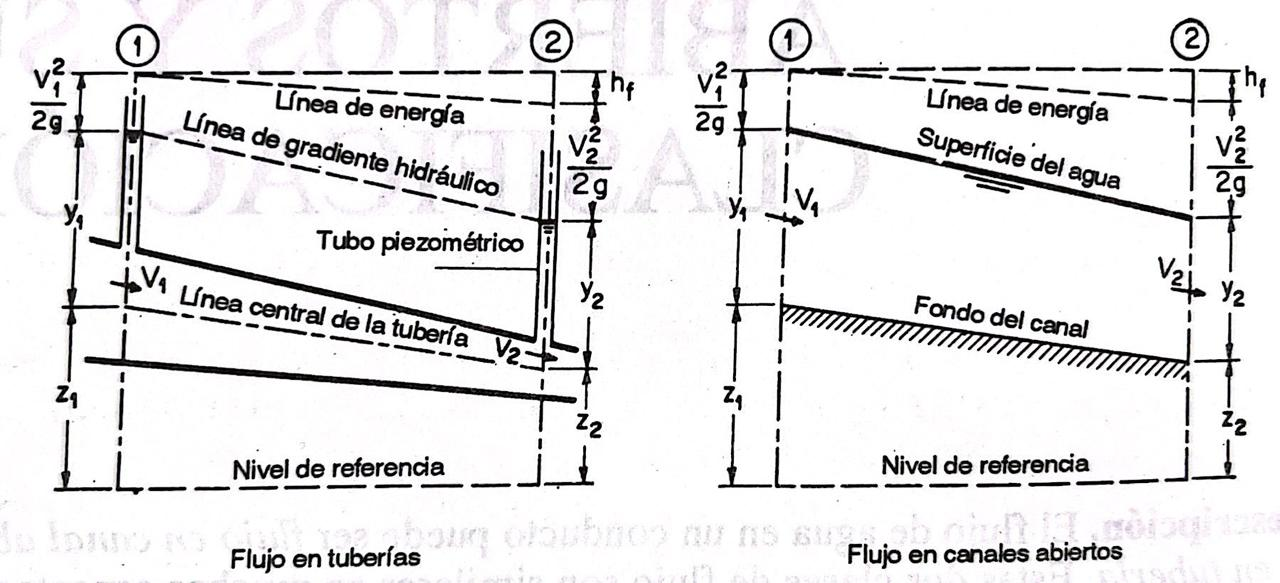
\includegraphics[width=8cm]{fig1.jpeg}
\caption{Linea de gradiente hidraulico y de energia en a) flujo a presi\'on y b) flujo a superficie libre (tomado de \cite{VChow}).}
\label{fig1}
\end{figure}

Cabe aclarar que el an\'alisis del flujo en canales es m\'as complejo que el flujo. Mientras que en una tuber\'ia la secci\'on que atravieza el flujo es constante y determinada por la geometr\'ia de la tuber\'ia que es muchas veces circular, en un canal la secci\'on puede tomar muchas formas geom\'etricas e inclusive puede ser totalmente irregular como en el caso de canales naturales. Por otro lado, la presi\'on en una tuber\'ia de secci\'on constante no cambia en el tiempo mientras que en un canal la profundidad  del flujo cambia cuando cambia la pendiente del canal. Esto hace que las pendientes de la superficie del agua y del fondo del canal sean diferentes. Ademas, mientras que la rugosidad en una tuber\'ia es independiente de las condiciones de flujo, la rugosidad en un canal depende del nivel de agua. Todos estos factores hacen que el flujo en canales sea m\'as incierto y recurra m\'as al uso de ecuaciones emp\'iricas y al conocimiento previo de otras disciplinas como la \emph{hidrolog\'ia} y la \emph{geomorfolog\'ia}.

\subsection{Tipos de canales}
Un canal es un conducto en el cual es agua fluye con su superficie libre (en contacto con la atmosfera). Los canales pueden ser clasificados como:
\begin{itemize}
\item \textbf{Naturales}: Son aquellos cursos naturales de agua que existen sobre la tierra. Se pueden clasificar como arroyos o quebradas que existen en zonas montañosas hasta rios y estuarios, los cuales poseen dimensiones mucho mayores y existen en llanuras y en desembocaduras a oceanos y mares, respectivamente. Dedido a su irregularidad, las propiedades hidr\'aulicas de los canales naturales cambian continuamente en el espacio y en el tiempo. 
\item \textbf{Artificiales}: Son aquellos construidos por el ser humano cuyas formas suelen ser de geometr\'ia conocida. Estos canales  se construyen para la navegaci\'on, en centrales hidroel\'ectricas, en sistemas de riego, en drenajes en v\'ias, para vertederos y tomas de agua, y en laboratorios para el estudio del flujo. Se han encontrado que las teor\'ias hidr\'aulicas desarrolladas para canales artificiales se pueden aplicar a canales naturales con un buen grado de aproximaci\'on.  Existen tipos de canales artificiales:

\begin{itemize}
\item \emph{Canal}: Canal excavado en el sitio generalmente revestido con pasto, concreto, ladrillo o asfalto. Usualmente tienen bajas pendientes y son utilizados en el drenaje urbano.
\item \emph{Canaleta}: Canal de menor tamaño que el canal y apoyado sobre el terreno. Suelen construirse en metal, mamposter\'ia o concreto y sirven para transportar el agua  a trav\'es de una depresi\'on. 
\item \emph{Rapidas y Caida}: Son canales de alta pendiente construidos en longitudes cortas. 
\item \emph{Alcantarilla}: Es un canal cerrado, generalmente de secci\'on circular y longitud corta, construido en concreto o mamposteria que sirve para el drenage de aguas servidas y lluvias en sistemas urbanos. 
\item \emph{T\'uneles}: Canales no revestidos y excavados en roca, y revestidos en concreto o mamposter\'ia comunmente usados en centrales hidroel\'ectricas. 
\end{itemize}
\end{itemize}

\begin{figure}[h]
\centering
%\includegraphics[width=8cm]{fig2.jpeg}
\caption{a) Canal artificial b) quebrada de alta montaña.}
\label{fig2}
\end{figure}

\begin{figure}
     \centering
     \begin{subfigure}[b]{0.45\textwidth}
         \centering
         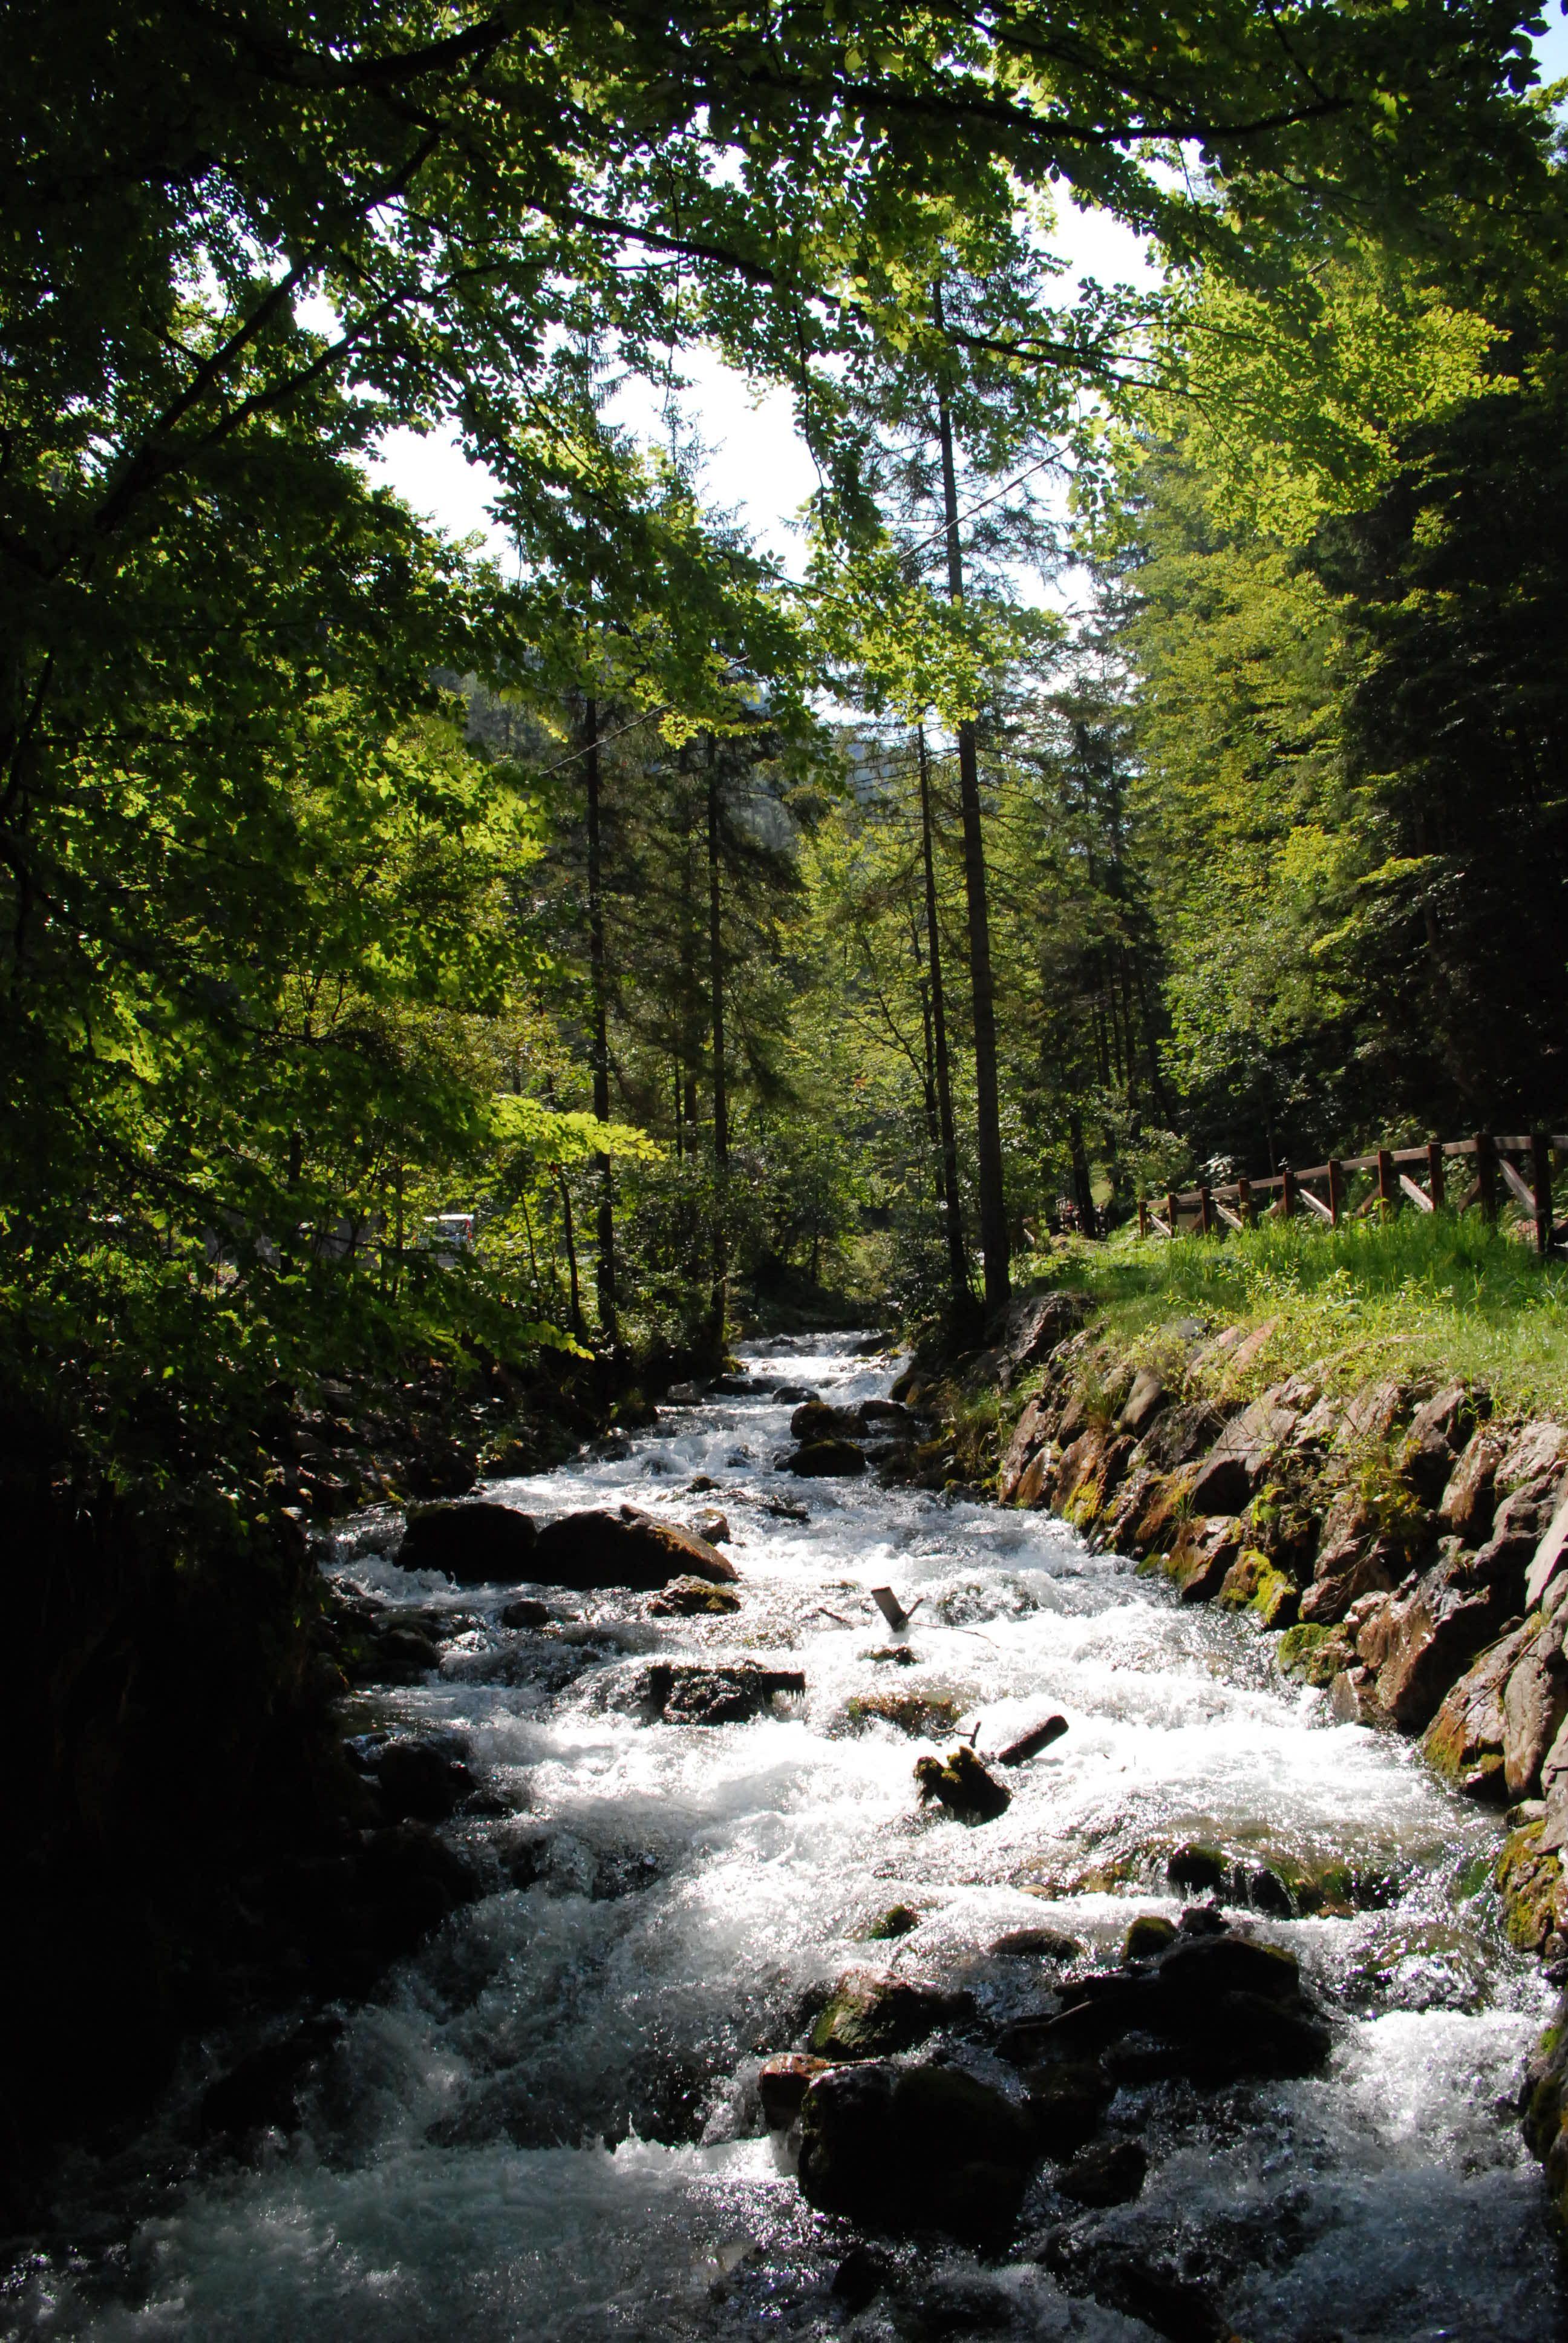
\includegraphics[width=\textwidth]{fig2a}
         \caption{Quebrada de alta montaña}
         \label{fig2a}
     \end{subfigure}
     \hfill
     \begin{subfigure}[b]{0.45\textwidth}
         \centering
         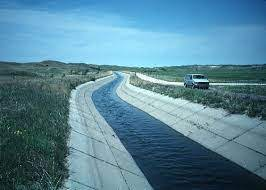
\includegraphics[width=\textwidth]{fig2b}
         \caption{Canal artificial}
         \label{fig2b}
     \end{subfigure}
      \caption{Tipos de canales principales.}
      %\label{fig:three graphs}
\end{figure}


\subsection{Geometr\'ia de un canal}
Un \emph{canal prismatico} es aquel cuya seccion transversal y pendiente permanecen constantes mientras que un \emph{canal no prismatico} es aquel en donde la seccion y/o la pendinte cambian a lo largo de su longitud (e.g. vertedero de ancho variable). La seccion de un canal, es la seccion en la dimension transversal o perpendicular a la direcci\'on de flujo. En  canales naturales la secci\'on transversal es irregular y cambia en el espacio y en el tiempo. Cuando ocurren crecientes, generalmente el canal central transporta la mayoria del flujo mientras los canales en las bancas transportan menor flujo.

Los canales artificiales tienen geometr\'ias como las que se muestran en la figura~\ref{fig3}. Los canales abiertos m\'as comunes son los rectangulares y los trapezoidales. Los canales circulares son los mas comunes en sistemas de alcantarillado. Existen otras formas de canales cerrados como la secci\'on rectangular, en forma de ovalo o de erradura. En muchos estudios de cauces naturales la par\'abola se utiliza como una aproximaci\'on a una secci\'on de un canal natural. 

% VChow fig 2.1
\begin{figure}[h]
\centering
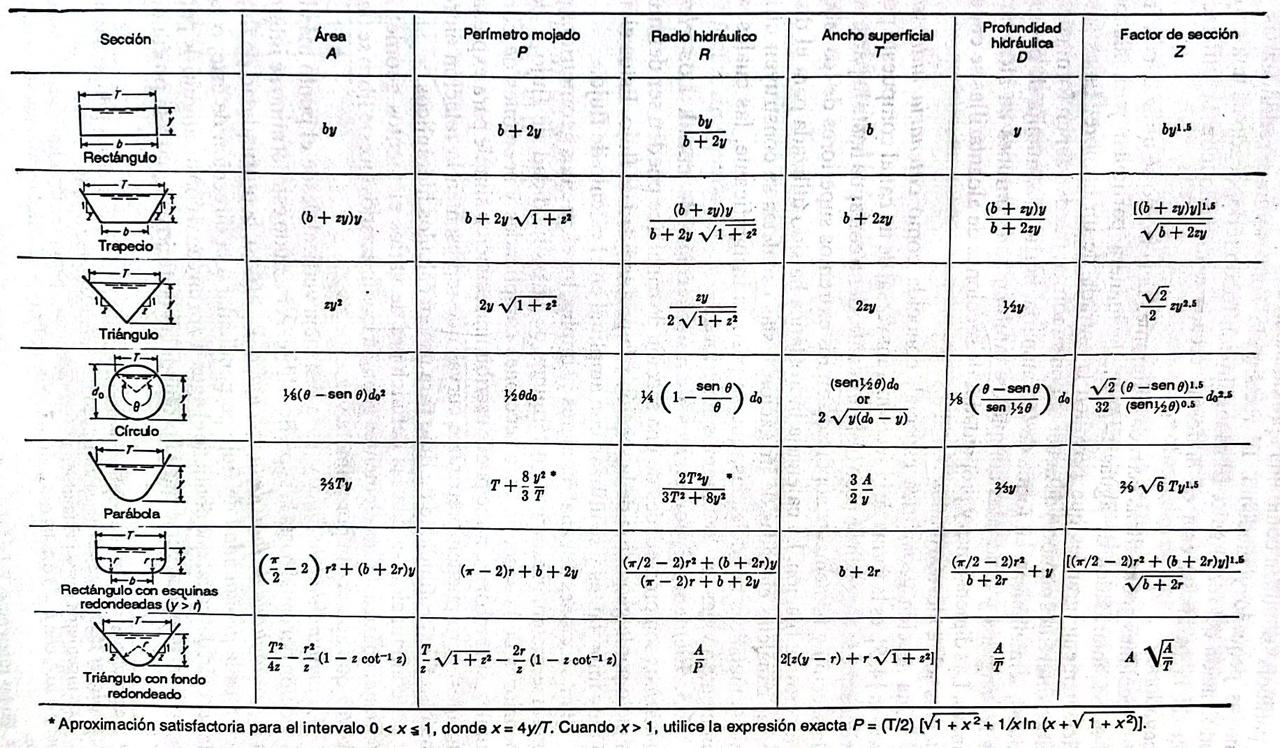
\includegraphics[width=8cm]{fig3.jpeg}
\caption{Geometr\'ias y elementos geom\'etricos de secciones transversales de un canal (tomado de \cite{VChow}).}
\label{fig3}
\end{figure}

Las \emph{propiedades geom\'etricas} (ver figura~\ref{fig3}) de un canal se expresan a traves de ecuaciones en funci\'on de la profundidad del flujo y de otras dimensiones de la secci\'on. Sin embargo para el caso de canales naturales, no es posible obtener ecuaciones y es necesario el uso de m\'etodos num\'ericos para obtener dichas propiedades. Las propiedades geom\'etricas mas importantes son las siguientes:
\begin{itemize}
\item \textbf{profundidad de flujo ($y$)}: es la distancia vertical desde el punto mas bajo de la secci\'on hasta la superficie del agua. 
\item \textbf{profundidad de la secci\'on ($d$)}: es la distancia perpendicular al flujo desde el punto mas bajo de la seccion hasta la sueperficie del agua. $y=\frac{d}{\cos \theta}$ donde $\theta$ es el angulo de la pendiente longitudinal del canal. 
\item \textbf{nivel ($z$)}: es la elevaci\'on de la superficie del agua desde un nivel de referencia o datum. Si el nivel de referencia es el fondo, $z=y$.
\item  \textbf{ancho superficial ($T$)}: ancho de la secci\'on transversal en la superficie libre. 
\item  \textbf{\'area mojada ($A$)}: es el \'area de la secci\'on transversal en contacto con el fluido perpendicular a la direcci\'on del flujo. 
\item  \textbf{perimetro mojada ($P$)}: es el per\'imetro de la secci\'on transversal en contacto con el fluido.
\item  \textbf{radio hidr\'aulico ($R$)}: es la relaci\'on entre el per\'imetro mojado y el \'area mojada, $R=\frac{A}{P}$.
\item  \textbf{profundidad hidr\'aulica ($D$)}: es  $D=\frac{A}{T}$.
\item  \textbf{factor de secci\'on ($Z$)}: para el c\'alculo del \emph{flujo cr\'itico}, se calcula como $Z= A\sqrt{D} = A \sqrt{\frac{A}{T}}$. Para el caso de \emph{flujo uniforme} $Z=AR^{(2/3)}$.
\end{itemize}

%%%%%%%%
\section{Clasificaci\'on y reg\'imenes de flujo} % From Chau 
Con base en diferentes criterios, el flujo a superficie libre se puede clasificar en diferentes tipos (ver figura~\ref{fig4}).

% Chau fig 1.7
\begin{figure}[h]
\centering
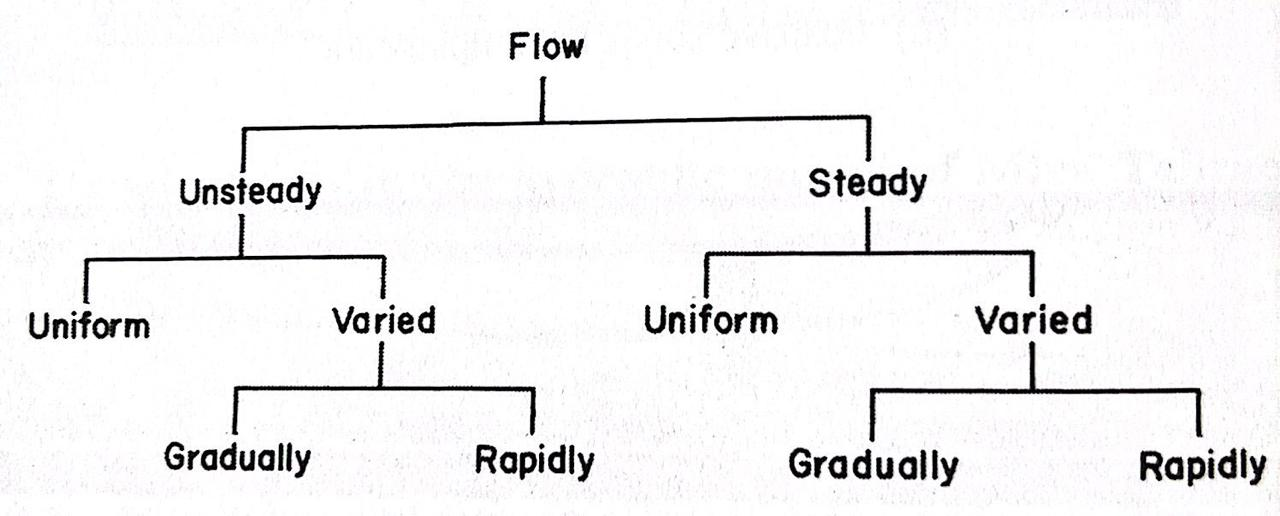
\includegraphics[width=8cm]{fig4.jpeg}
\caption{Clasificaci\'on de flujos a superficie libre (tomado de \cite{Chau}).}
\label{fig4}
\end{figure}

\subsection{Flujo permanente y no permanente}
Si la velocidad del flujo ($\vec{U}= u\vec{i} + v\vec{j} + w\vec{k}$) en un punto determinado del espacio dentro del flujo no cambia en el tiempo $t$, el flujo es \emph{permanente}. Si la velocida del flujo cambia en un punto determinado del espacio con respecto al el tiempo, el flujo es no \emph{permanente}. Esto quiere decir que el termino de la \emph{aceleracion local} ($\partial{\vec{U}}/\partial{t}$), en el campo vectorial de la aceleracion ($\vec{a}$), es igual a cero (el cambio de las tres componentes de $\vec{U}$ con respecto al tiempo es cero). Es posible transformar el flujo no permanente en flujo permanente si el sistema de referencia se mueve con el flujo, e.g. con una onda de creciente que no cambia de forma.  

\subsection{Flujo uniforme y no uniforme}
Si la velocidad del flujo para un instante de tiempo $t$ no cambio a lo largo de un tramo de canal ($\vec{l} = x\vec{i} + y\vec{j} + z\vec{k}$), el \emph{flujo es uniforme}. Esto quiere decir que el \emph{termino convectivo} ($\vec{U} ( \vec{\nabla} \cdot \vec{U} )$) del  campo vectorial de la aceleraci\'on es igual a cero. Note que el operador $\vec{\nabla}=\frac{\partial}{\partial x} \vec{i} + \frac{\partial}{\partial y} \vec{j} + \frac{\partial}{\partial z} \vec{k}$. Esta condici\'on de flujo uniforme se cumple para la velocidad media de una secci\'on. Sin embargo se considera flujo uniforme incluso cuando la velocidad en diferentes puntos de una secci\'on no es la misma. 

Cuando la velocidad para un instante de tiempo dado cambia a lo largo de un tramo de canal, el flujo se considera \emph{no uniforme} o \emph{variado}. Dependiendo de la variacion a lo largo del canal, el flujo se puede clasificar como \emph{gradualmente variado} o \emph{rapidamente variado}. En un flujo fradualmente variado, la profundidad de flujo varia gradualmente a lo largo de la distancia mientras que en un flujo rapidamente variado la profundidad varia rapidamente para una distancia corta.

De acuerdo con lo anterior, para flujo permanente y uniforme, la velocidad no varia ni con con el espacio ni con el tiempo, esto quiere decir que el campo vectorial de la aceleracion (derivada total de la velocidad con respecto al tiempo) es igual a cero $\vec{a}=\frac{d \vec{U}}{d t} = 0$.

\subsection{Flujo laminar y flujo turbulento}
El flujo es \emph{laminar} cuando las particulas de fluido se desplazan de manera organizada formando capas que se mueven unas sobre otras. En un flujo \emph{turbulente} las particulas de fluido se mueven de manera ca\'otica en trayectorias irregulares. Analizando las fuerzas que intervienen en el flujo de fluidos, el flujo es laminar cuando las fuerzas dominantes son las \emph{fuerzas viscosas} y es turbulento cuando las fuerzas dominantes son las \emph{fuerzas inerciales}. La clasificaci\'on de un flujo en laminar o turbulento, se hace a trav\'es del \emph{numero de Reynolds} ($R_e$):
\begin{equation}
R_e = \frac{\text{fuerzas inerciales}}{\text{fuerzas viscosas}} = \frac{V L}{\nu}
\label{Re}
\end{equation}
donde $V$ es la velocidad media de la secci\'on, $\nu$ es la viscosidad cinem\'atica del fluido y $L$ es una longitud caracteristica que para flujo a superficie libre es igual al radio hidraulico $R$ o la profundidad hidraulica. Para flujo en canales, la transicion de flujo laminar a turbulento ocurre cuando $R_e \approx $ 600. Flujo laminar a superficie libre es muy raro en la vida real. Sin embargo en modelos a escala, es posible que para profundidades de flujo pequeñas  se presente flujo laminar en el modelo cuando en realidad el flujo en el prototipo es turbulento. 

\subsection{Flujo subcr\'tico, cr\'itico y supercr\'itico}
Un flujo es \emph{cr\'itico} cuando este tiene una velocidad media igual a la velocidad con la que se desplaza una onda de gravedad de pequeña amplitud en el flujo. La onda de gravedad se forma por cambios en la profundidad del flujo. Un flujo es \emph{subcr\'itico} cuando la velocidad media es menor que la \emph{velocidad cr\'tica} y es \emph{supercr\'itico} cuando la velocidad media es mayor que la velocidad critica. Para la clasificaci\'on de estos tipos de flujo, se utiliza el \emph{n\'umero de Froude} ($R_r$):
\begin{equation}
F_r = \frac{\text{fuerzas inerciales}}{\text{fuerzas gravitacionales}} = \frac{V}{\sqrt{g L}}
\label{Fr}
\end{equation}
donde $g$ es la aceleraci\'on de la gravedad y $L$ es una longitud caracteristica igual a la profundidad hidraulica $D$ que para canales rectangulares es $D=y$. De acuerdo con la ecuacio~\ref{Fr}, el flujo es cr\'tico cuando $F_r = 1$, es subcr\'itico cuando $F_r < 1$ y es supercritico cuando $F_r > 1$.

Pueden presentarse combinaciones de tipos de flujo de acuerdo con el valor de $R_e$ y de $F_r$ como: \emph{subcritico laminar}, \emph{subcritico turbulento}, \emph{supercritico laminar} y \emph{supercritico turbulento} (ver figura~\ref{fig41})

% VChow fig 1.5
\begin{figure}[h]
\centering
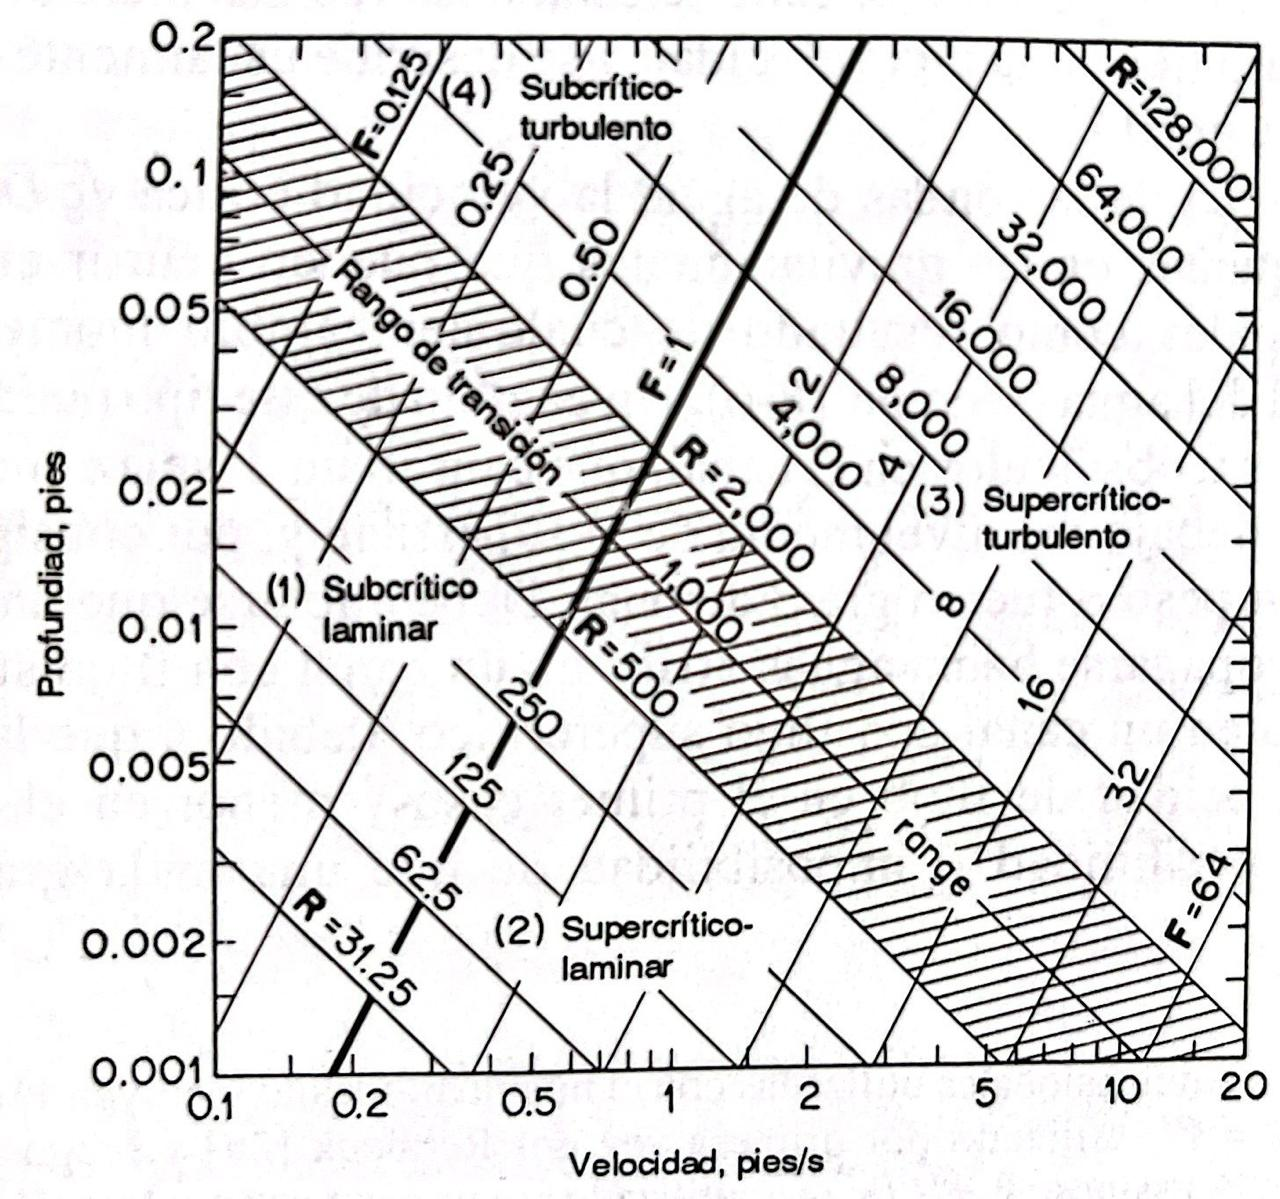
\includegraphics[width=8cm]{fig41.jpeg}
\caption{Profundidad vs velocidad para cuatro regimenes flujo en canales abiertos anchos. Note que las escalas son logaritmicas (tomado de \cite{VChow}).}
\label{fig41}
\end{figure}

Los flujos subcritico laminar y supercritico laminar son poco comunes en la naturales y se presentan cuando la profundidad de agua es pequeña lo cual suele ocurrir en modelos a escala. En casos reales los flujos son turbulentos.

%%%%%%%%
\section{Distribuci\'on de velocidades}% From Chau 
La velocidad del flujo en una seccion de canal varia en cada punto dentro de esta debido a los esfuerzos cortantes entre capas de flujo inducidas por la rugosidad ejercida por el fondo y las bancas del canal, y por la superficie libre en contacto con el aire (ver figura~\ref{fig5}).

% Chau fig 1.9
\begin{figure}[h]
\centering
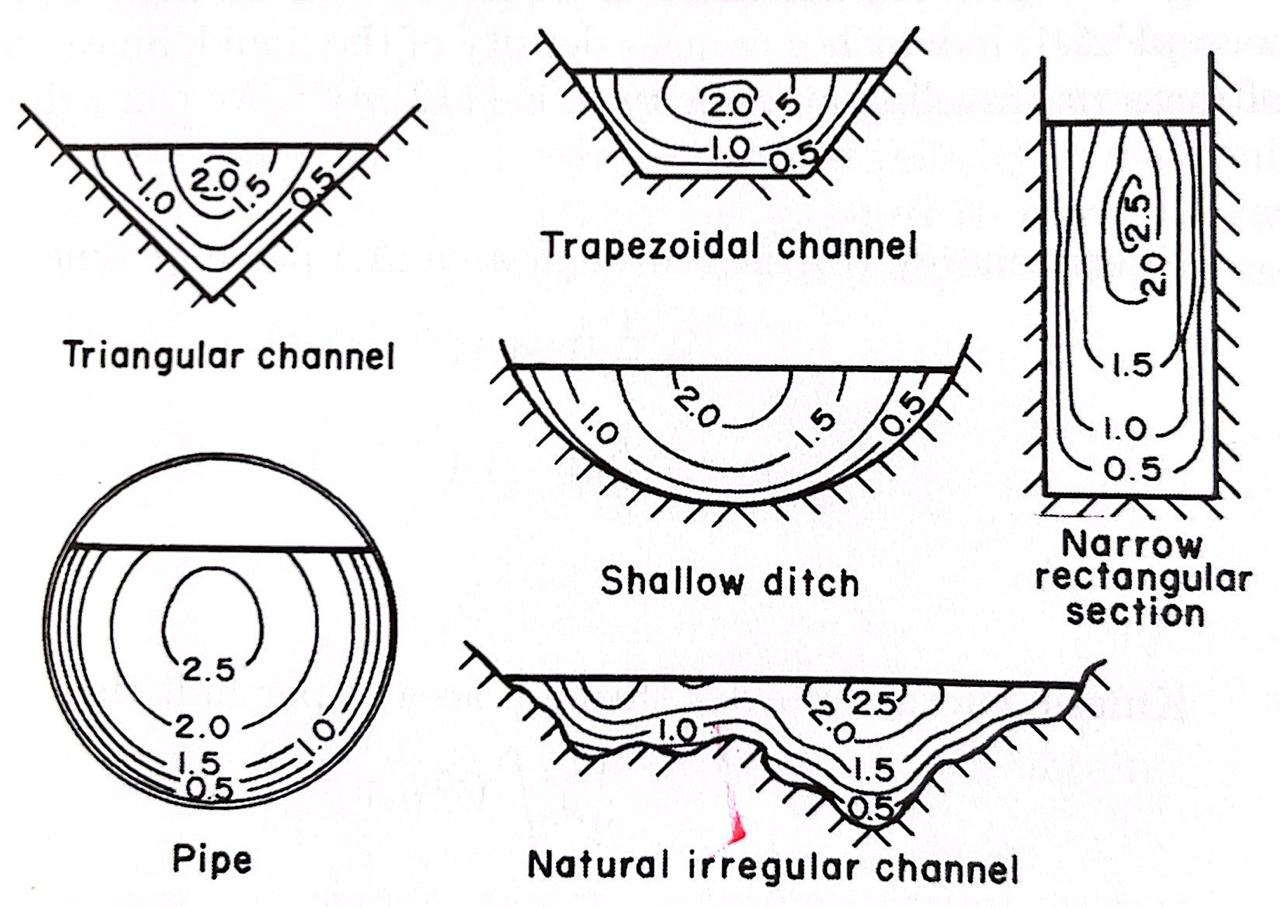
\includegraphics[width=8cm]{fig5.jpeg}
\caption{Distribuci\'on de velocidad de flujo en diferentes tipos de canales (tomado de \cite{Chau}).}
\label{fig5}
\end{figure}


En teoria la velocidad varia en las tres dimensiones espaciales. Sin embargo en la practica, los mayores gradientes de velocidad se dan a lo largo de la direccion del flujo. 
% VChow fig 2.5
\begin{figure}[h]
\centering
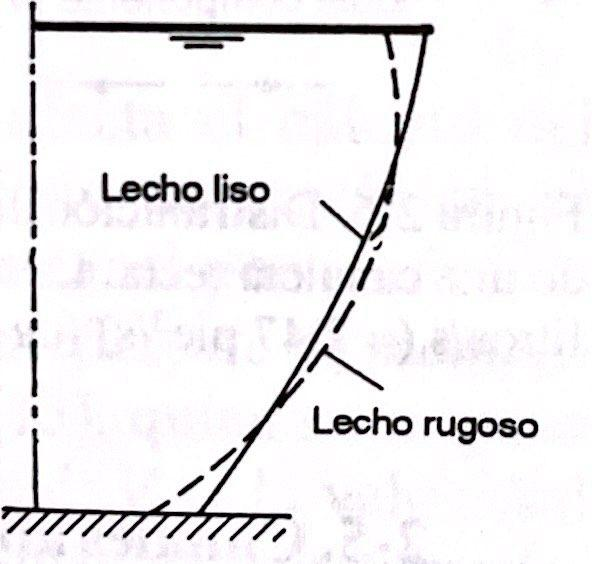
\includegraphics[width=8cm]{fig6.jpeg}
\caption{Distribuci\'on de velocidades en un canal liso y rugoso (tomado de \cite{VChow}).}
\label{fig6}
\end{figure}

\subsection{Coeficiente de energ\'ia}
%Teniendo en cuenta que la velocidad cambia en cualquier punto en una seccion transversal de un canal, la cabeza de velocidad promedio ($\left( \frac{U^2}{2g} \right)_m$) es diferente a la ccabeza de velocidad estimada con la velocidad media ($\frac{V^2}{2g}$). 
Si analizamos un flujo de fluido de densidad $\rho$ cuyo campo de velocidades es $\vec{U}$ que pasa a traves de una seccion infinitesimal $dA$, la energ\'ia cinem\'atica del flujo por unidad de tiempo es $\frac{1}{2}\rho dA U^3$. La energ\'ia cinem\'atica del flujo a partir de la velocidad media en la seccion $V$, se puede estimar como  $\frac{1}{2}\rho dA V^3$. Sin embargo estas dos maneras de calcular la energ\'ia cinem\'atica por unidad de tiempo no son equivalentes. Para superar estas diferencias, se introduce un \emph{coeficiente de energia} o \emph{coeficiente de Coriolis} en la seguanda ecuacion, quedando $\frac{1}{2}\alpha \rho dA V^3$. Igualando las dos ecuaciones e integrando para el area $A$ de la seccion transversal, se tiene:

$$
\frac{1}{2}\alpha\rho V^3 \int_A dA  = \frac{1}{2}\rho \int_A U^3 dA 
$$
Simplificando y despenjando para $\alpha$, se tiene que:

\begin{equation}
\alpha = \frac{\int_A U^3 dA}{V^3 \int_A dA}
\label{alp}
\end{equation}

Teniendo en cuenta que la velocidad media en la secci\'on de flujo $V$ se calcula como $V=\frac{1}{A}\int_A U dA$, reemplazando en la ecuaci\'on~\ref{alp}, tenemos:

\begin{equation}
\alpha = \frac{A^3 \int_A U^3 dA}{\left(\int_A U dA \right)^3 \int_A dA}= \frac{A^2 \int_A U^3 dA}{\left(\int_A U dA \right)^3 }
\label{alp2}
\end{equation}

La forma discreta de la ecuaci\'on anterior, se expresa como:

\begin{equation}
\color{red}\boxed{\color{black} \alpha = \frac{\sum_{i=1}^{N}A_i^2 \sum_{i=1}^{N} U_i^3 A_i} {\left(\sum_{i=1}^{N} U_i A_i \right)^3 }}
\label{alp3}
\end{equation}

donde $N$ es el numero de subsecciones verticales en las cuales una secci\'on es dividida, $A_i$ es el area de la subsecci\'on $i$ y $U_i$ es la velocidad media en la subsecci\'on $i$.

\subsection{Coeficiente de cantidad de movimiento}
El flujo de cantidad de movimiento por unidad de tiempo a trav\'es de una secci\'on $dA$ cuyo campo de velocidad es $\vec{U}$ es $\frac{1}{2}\rho dA U^2$. Si tomamos la velocidad media en la secci\'on $V$, el flujo de cantidad de movimiento a trav\'es de $dA$ por unidad de tiempo es $\frac{1}{2}\rho dA V^2$. Para que estas dos ecuaciones sean equivalentes, la \'ultima ecuaci\'on se debe multiplicar por un \emph{coeficiente de cantidad de movimiento} ($\beta$), quedando $\frac{1}{2}\beta \rho dA V^2$. Igualando estas dos ecuaciones e integrando para $A$, se tiene:

$$
\frac{1}{2}\beta\rho V^2 \int_A dA  = \frac{1}{2}\rho \int_A U^2 dA 
$$

Simplificando y despenjando para $\alpha$, se tiene que:
\begin{equation}
\beta = \frac{\int_A U^2 dA}{V^2 \int_A dA}
\label{bet}
\end{equation}

Reemplazando para $V$ en la ecuaci\'on~\ref{bet}, se tiene:
\begin{equation}
\beta = \frac{A \int_A U^2 dA}{\left(\int_A U dA \right)^2 }
\label{bet2}
\end{equation}

La forma discreta de la ecuaci\'on anterior, se expresa como:

\begin{equation}
\color{red}\boxed{\color{black} \beta = \frac{\sum_{i=1}^{N}A_i \sum_{i=1}^{N} U_i^2 A_i} {\left(\sum_{i=1}^{N} U_i A_i \right)^2 }}
\label{bet3}
\end{equation}

Valores teoricos de $\alpha$ y $\beta$ se pueden deducir a partir de la \emph{ley de potencia} o de la \emph{ley logaritmica} de distribuci\'on de velocidades en canales anchos. Algunos valores tipicos de $\alpha$ y $\beta$ para diferentes secciones de canal, se relacionan la tabla~\ref{tab1}. En terminos generales para canales prismaticos y circulares rectos, los valores de $\alpha$ y $\beta$ son menores a 1.15 y aproximadamente igual a 1.0.

% Chau tab 1.2
\begin{table}[h!]
\centering
\begin{tabular}{l c c}
 \hline
 Secci\'on de canal & $\alpha$ & $\beta$ \\ [0.5ex]
 \hline\hline
Canales regulares & 1.10-1.20 & 1.03-1.07 \\
Canales naturales & 1.15-1.50 & 1.05-1.17 \\
Rios cubiertos de hielo & 1.20-2.00 & 1.07-1.33 \\
Llanuras de inundacion & 1.50-2.00 & 1.17-1.33 \\
\hline
\end{tabular}
\caption{Coeficientes $\alpha$ y $\beta$ para diferentes tipos de secci\'on (tomado de \cite{Chau}).}
\label{tab1}
\end{table}

%%%%%%%%
\section{Distribuci\'on de presiones}% From Chau 
La distribuci\'on de presiones en un canal depende de las condiciones de flujo. A continuacion se analisara las distribuciones para diferentes condiciones.

\subsection{Fluido est\'atico}
En el caso de un fluido estatico, si se analizan las fuerzas ejercidas sobre una porci\'on del fluido de area transversal $dA$ y altura $y$, se tiene que las fuerzas en el plano horizontal se cancelan, por lo que las unicas fuerzas actuantes son el eje vertical $z$. Haciendo sumatoria de fuerzas en $z$ igual a zero (fluido estatico sin aceleraci\'on) y trabajando en terminos de presiones manometricas, tenemos que:
$$
f_z = w
$$
donde $w$ es el peso del elemento de fluido fluido $W=\rho g y dA$ y $f_z$ es la fuerza de presi\'on hidroestatica $p$ ejercida  por el fluido sobre $dA$ por lo que $f_z = p dA$. Reemplanzando y simplificando, tenemos:

$$
p=\rho g y
$$
Esta ecuaci\'on determina la presi\'on manometrica en un fluido incompresible ($\rho$ es constante) en reposo a una profundidad $y$. Note que a grandes profundidades $\rho$ cambia por lo que la ecuaci\'on anterior no se cumple.

\subsection{Flujo horizontal y paralelo}
Consideremos ahora un fluido que se mueve en capas en un canal horizontal sin fricci\'on. Si  no existe aceleracion del fluido en la direcci\'on del flujo y si la velocidad es uniforme en la secci\'on y paralela al fondo del canal, la sumatoria de fuerzas en la direcci\'on del flujo es cero. Las fuerzas actuantes son a lo largo del eje vertical las cuales son la fuerza de presi\'on hidroestatica a una profundidad $y$ y el peso del elemento de fluido $w$. Similar al caso de fluido est\'atico, tenemos entonces que:

$$
p=\rho g y
$$
 
\subsection{Flujo paralelo en un canal inclinado}
Consideremos el flujo en un canal con una pendiente dada por el angulo $\theta$ (ver figura~\ref{fig7}). Si no existe aceleracion del fluido en direcci\'on del flujo y si la velocidad es uniforme en la secci\'on del canal y paralela al fondo de este, las fuerzas actuantes son a lo largo del eje del elemento y su sumatoria es igua a cero. El peso  $w=\rho g d dA$ en direcci\'on vertical hacia abajo, al proyectarlo sobre el eje del elemento se tiene $w=\rho g dA \cos \theta d$; note que $d$ es la profundida de la seccion. La otra fuerza a lo largo del eje del elemento es la fuerza de presi\'on $f_z=p dA$. Teniendo en cuenta que $d= y \cos \theta$, el peso del elemento de fluido se convierte en $w = \rho g y \cos^2 \theta$. Haciendo sumatoria de fuerzas a lo largo del eje del elemento, se tiene:

$$
p=\rho g y \cos^2 \theta
$$

% Chau fig 1.15
\begin{figure}[h]
\centering
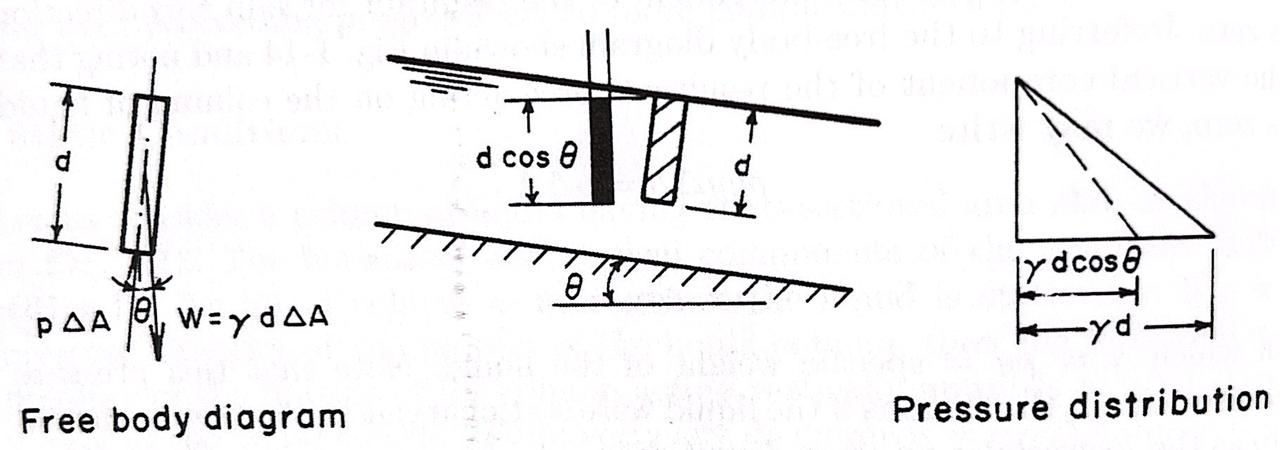
\includegraphics[width=8cm]{fig7.jpeg}
\caption{Fuerzas actuantes sobre un elemento de flujo en un canal con pendiente (tomado de \cite{Chau}).}
\label{fig7}
\end{figure}


La ecuacion anterior muestra que la presi\'on en el fluido no es hidroestatica como en los dos casos anteriores. Sin embargo para casos practicos la pendiente del canal es relativamente pequeña por lo que $\cos \theta \approx 0$. Esto implica que $d \approx y$. La ecuacion anterior queda entonces:

$$
p \approx \rho g y \approx \rho g d
$$
La ecuacion anterior es de nuevo la presi\'on hidroestatica que para el caso en cuestion es aplicable considerando un canal de pendiente pequeña. La presi\'on hidroestativa es aplicable en flujo uniforme y flujo variado.


\subsection{Flujo curvilineo}
En los casos anteriores se asumio que la velocidad era uniforme en la seccion y paralela al fondo. Sin embargo, existen muchos casos en los que las lineas de flujo se curvan lo cual cambia la distribuci\'on de presiones en un elemento de flujo debido a fuerzas centrifugas perpendiculares a la direcci\'on del flujo. Para este caso, consideremos las fuerzas verticales actuantes sobre un elemento de flujo (ver figura~\ref{fig8}).

% Chau fig 1.16
\begin{figure}[h]
\centering
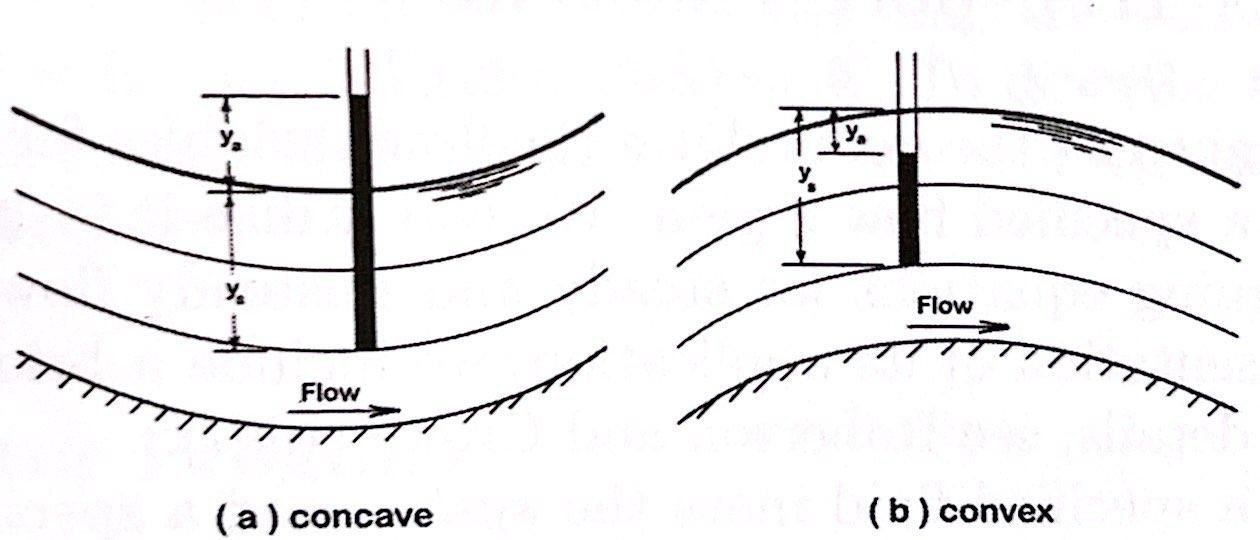
\includegraphics[width=8cm]{fig8.jpeg}
\caption{Fuerzas actuantes sobre un elemento de flujo curvilineo (tomado de \cite{Chau}).}
\label{fig8}
\end{figure}

Si la curvatura de las lineas de flujo es $r$ y la velocidada en un punto es  $V$, tenemos que la $\text{aceleracion centrifuga}= \frac{V^2}{r}$ y la $\text{fuerza centrifuga}= \rho y_s dA \frac{V^2}{r}$ donde $y_s$ es la altura hidroestatica, $y_a$ es la correccion de la altura de presi\'on por curvatura y $h = y_s \pm y_a$ es la altura piezometrica. En el caso de flujo convexo las fuerzas actuan hacia arriba y la altura piezometria $h = y_s-y_a$; en el caso del flujo concavo, la altura piezometrica es $h = y_s+y_a$. $y_a$ se calcula a partir de la fuerza centrifuga:
$$
y_a = \frac{1}{g}y_s \frac{V^2}{r}
$$

La altura piezometrica se calcula entonces como:
$$
h = y_s \left( 1 \pm \frac{1}{g} \frac{V^2}{r} \right)
$$

Note que $h$ representa la cabeza de energia de presi\'on. 

\begin{alg}{Calculo de los coeficientes de energia y de cantidad de momvimiento}{alg1}
\begin{enumerate}
\item Leer la siguiente informaci\'on: $l$, $xs$, $ys$ y $Vs$. Note que $xs$ y $ys$ son dos vectores con las coordenadas $x$ y $y$ respectivamente para un numero $m$ de puntos que conforman la seci\'on transversal. $Vs$ es un vector de velocidades medias de $m-1$ segmentos que conforman la seccion.
\item Con base en las coordenadas datas ($xs$ y $ys$), interpolar un nuevo conjunto de puntos para el nivel $l$.   
\item Calcular el area de cada segmento de area $A_i$, con base en el nuevo conjunto de puntos ($xs$ y $ys$).
\item Con base en los valores de $A_i$ y de $Vs$, calcular el coeficiente de energ\'ia ($\alpha$) con la ecuaci\'on~\ref{alp3} y el coeficiente de cantidad de movimiento ($\beta$) usando la ecuaci\'on~\ref{bet3}.
\item Imprimir: Coeficiente de energ\'ia ($\alpha$) y el coeficiente de cantidad de movimiento ($\beta$). 
\end{enumerate}
\end{alg}

\begin{eje}{}{eje1}
  For all natural number $n$ it holds:
\end{eje}


%%%%%
\section{Conservacion de la energ\'ia}% From VChow
La energia total del flujo ($H$) en un punto $A$ de una secci\'on transversal de canal en unidades de fuerza por unidades de longitud sobre unidades de fuerza, con respecto a un nivel de referencia (ver figura~\ref{fig9}), est\'a dada por ecuaci\'on:

% VChow fig 3.1
\begin{figure}[h]
\centering
%\includegraphics[width=8cm]{fig9.jpeg}
\caption{(tomado de \cite{VChow}).}
\label{fig9}
\end{figure}

\begin{equation}
H = z_{A} + d_{A} \cos \theta + \frac{U_A^2}{2g} 
\label{ene1}
\end{equation}

donde $z_A$ es el  nivel de un elemento de fluido $A$ contenido en una linea de corriente con respecto a un nivel de referencia, $d_A$ es la profundidad del elemento de fluido $A$ medida desde la superficie libre, $\theta$ es el angulo de inclinaci\'on del canal y $V_A$ es la velocidad de flujo en el punto $A$. Para efectos pr\'acticos, la distribuci\'on de velocidades en la secci\'on se considera uniforme, por lo que el termino de la cabeza de energ\'ia cinetica de  la ecuaci\'on~\ref{ene1} se corrige utilizando el coeficiente de energ\'ia ($\alpha$) para tener en cuenta la distribuci\'on no uniforme de velocidades en la secci\'on. Para una secci\'on cualquiera, tenemos:

\begin{equation}
\color{red}\boxed{\color{black} H = z + d \cos \theta + \alpha\frac{V^2}{2g} }
\label{ene2}
\end{equation}

donde $z$ es el nivel del fondo del canal y representa la \emph{cabeza de energ\'ia potencial} del flujo, $d$ es la profundidad de la secci\'on medida perpendicular desde la superficie hasta el fondo del canal y representa la \emph{cabeza de energ\'ia de presi\'on} y $V$ es la velocidad media en la secci\'on. El t\'ermino $\alpha \frac{V^2}{2g}$ representa la \emph{cabeza de energ\'ia cin\'etica} corregida del flujo. Si $\theta \approx 0$, el termino $d \cos \theta \approx d = y$, donde $y$ es la profundidad del flujo. 

Analizando la figura~\ref{fig9} y teniendo en cuenta que la ecuacio\'on~\ref{ene2} representa la energ\'ia en una secci\'on del canal, la pendiente de la l\'inea energ\'ia conocidada como \emph{gradiente de energ\'ia} se representa como $S_f=\frac{h_f}{L}$ donde $h_f$ es la perdida de energia entre dos secciones y $L$ es la distancia horizontal entre las secciones. Para el caso de \emph{flujo uniforme} la pendiente de la linea de energ\'ia ($S_w$) y la pendiente del fondo del canal ($S_o \approx \sin \theta$) son iguales al gradiente de energ\'ia: $S_f = S_w = S_o = \sin \theta$. Note que $\tan \theta \approx \sin \theta$ cuando $\theta \approx 0$. 

De acuerdo con el principio de conservacion de energ\'ia, la energ\'ia total entre dos secciones 1 y 2, se representa como:

\begin{equation}
z_1 + d_1 \cos \theta + \alpha_1 \frac{V_1^2}{2g} = z_2 + d_2 \cos \theta + \alpha_2 \frac{V_2^2}{2g} + h_{f}
\label{ene3}
\end{equation}

Para un canal con pendiente peque\~na, se tiene:

\begin{equation}
 z_1 + d_1 + \alpha_1 \frac{V_1^2}{2g} = z_2 + d_2 + \alpha_2 \frac{V_2^2}{2g} + h_{f}
\label{ene4}
\end{equation}

Si $\alpha_1 \approx \alpha_2 \approx 1$ y $h_f \approx 0$, la ecuaci\'on~\ref{ene4} se convierte en la \emph{ecuaci\'on de Bernoulli}:

\begin{equation}
\color{red}\boxed{\color{black} z_1 + d_1 + \frac{V_1^2}{2g} = z_2 + d_2 + \frac{V_2^2}{2g} = \text{constante}}
\label{ene5}
\end{equation}

\subsection{Energ\'ia espec\'ifica}
La \emph{energ\'ia espec\'ifica} en la secci\'on de un canal es la energia por unidad de fuerza con respecto al fondo del canal($z=0$). A partir de la ecuaci\'on~\ref{ene2}, se tiene:

\begin{equation}
\color{red}\boxed{\color{black} E =   d\cos \theta + \alpha\frac{V^2}{2g}}
\label{ene6}
\end{equation}

Cuando $\theta \approx 0$ y $\alpha = 1$, la ecuaci\'on anterior queda:
 
\begin{equation}
\color{red}\boxed{\color{black} E =   y  + \frac{V^2}{2g} = y + \frac{Q^2}{2g A^2 }}
\label{ene7}
\end{equation}

donde $Q$ es el caudal medio que pasa a trav\'es de la secci\'on del canal y $A$ es el area transversal de la secci\'on del canal. La ecuaci\'on~\ref{ene7} muestra que la energ\'ia espec\'ifica en la secci\'on de un canal es igual a la profundidad de flujo m\'as la cabeza de energ\'ia cinetica del flujo. Note que si $Q$ es conocido, la ecuaci\'on~\ref{ene7} se convierte en  una  funcion $y$.

Graficando la ecuaci\'on~\ref{ene7} se tiene la \emph{curva de energ\'ia especifica} (ver figura~\ref{fig10}), en donde las absisas estan representadas por $E$ y las ordenadas por $y$.
% VChow fig 3.2
\begin{figure}[h]
\centering
%\includegraphics[width=8cm]{fig10.jpeg}
\caption{Curva de energ\'ia especifica (tomado de \cite{VChow}).}
\label{fig10}
\end{figure}

Esta curva tiene dos asintotas: $y=0$ y $y=E$ (curva OD) para los cuales los cuales $E$ tiende a infinito. Note que para canales horizontales, la curva OD forma un angulo de 45$^o$. Para canales de alta pendiente, la asintota es $y=E=d \cos \theta$, por lo que el angulo es igual a $\cos \theta$. La curva ademas evidencia lo siguiente:
\begin{itemize}
\item Para un valor de $E$ existen dos posibles valores de $y$: $y_1$ y $y_2$. Estan dos profundidades son conocidas como las \emph{profundidades alternas}.
\item El valor minimo de la energ\'ia $E$ ocurre en el punto $C$. La profundidad alli es una sola y se conoce como la \emph{profundidad cr\'itica} ($y_c$). El flujo para $y_c$ tiene una \emph{velocidad cr\'itica} ($V_c$). 
\item Cuando $y > y_c$, la velocidad del flujo ($V$) es mayor que $V_c$ y por lo tanto el flujo es \emph{supercritico}. Cuando $y < y_c$, la velocidad del flujo ($V$) es menor que $V_c$ y por lo tanto el flujo es \emph{subcritico}.
\item Si el caudal aumenta en la ecuaci\'on~\ref{ene7}, la curva de energ\'ia espec\'ifica se desplaza hacia la derecha, si disminuye se desplaza hacia la izquierda. 
\end{itemize}


\subsection{Flujo critico}
El \emph{flujo critico} se define como aquel flujo para el cual el n\'umero de Froude ($F_r$) es igual a 1. Tambi\'en se puede definir como el flujo para el cual la energ\'ia espec\'ififa es minima. Teniendo en cuenta que $E=f(y)$, la energ\'ia espec\'ifica minima o critica, puede encontrar derivando la ecuaci\'on~\ref{ene7} con respecto a $y$:
$$
\frac{dE}{dy} = 1 - \frac{Q^2}{gA^3} \frac{dA}{dy} = 1 - \frac{V^2}{gA} \frac{dA}{dy}
$$
donde $\frac{dA}{dy} \approx T$, donde $T$ es el ancho superficial de la secci\'on. Teniendo en cuenta que $A/T$ es conocida como la profundidad hidraulica, tenemos:
$$
\frac{dE}{dy} = 1 -  \frac{V^2 T}{gA} = 1 -  \frac{V^2}{gD} 
$$
Si la energia es minima cuando  $\frac{dE}{dy}=0$, la expresi\'on anterior queda:

\begin{equation}
\frac{V^2}{2g} = \frac{D}{2} 
\label{ene8}
\end{equation}

Esta ecuaci\'on indica que la cabeza de energ\'ia cinem\'atica es igual a la mitad de la profundidad hidraulica para flujo critico. La ecuaci\'on anterior tambien se puede expresar como $\frac{V}{\sqrt{gD}}=1$ el cual es ecuacion de $F_r$ para flujo critico. La ecuaci\'on~\ref{ene8} se aplica para el caso de canales con pendiente baja y $\alpha = 1$. Para canales con pendiente alta y valores de $\alpha \ne 1$, la ecuaci\'on~\ref{ene8} se convierte:

\begin{equation}
\alpha \frac{V^2}{2g} = \frac{\cos \theta D}{2} 
\label{ene9}
\end{equation}

\subsection{Fen\'omenos locales}
Los fenomenos locates ocurren frecuentement en canales cuando hay cambios de regimen (de subcritico a supercritico o viseversa) en distancias. Existen dos tipos principales:
\begin{itemize}
\item \emph{Caida hidraulica}: Se presenta cuando hay un cambio brusco de la pendiente del fondo del canal lo cual hace que el flujo pase de ser subcritico a supercritico en una secci\'on de transicion en donde se presenta el la profunidad critica. 
\item \emph{Caida libre}: La caida libre se presenta cuando el fondo del canal cambia abrudtamente, como por ejemplo, en la descarga libre de un canal a un lago. En la caida libre, el flujo va de flujo subcritico antes de la caida alcanzando su energia minima justo en la secci\'on de la descarga. Sin embargo, analisis experimentales han encontrado que la secci\'on de energ\'ia critica no es examenente en la secci\'on de la descarga debido a la curvatura de la lamina de agua por lo que para pendientes pequeñas $y_c = 1.4 y_o$, donde $y_o$ es la profundidad en el borde y $y_c$ se localiza entre 3 y 4 $y_c$ aguas arriba del borde del canal.
\item \emph{Resalto hidr\'aulico}: Se presenta cuando existe un aumento rapido de la lamina de agua que puede ser causado aguas abajo del flujo bajo una compuerta  en un canal horizontal, o al final de un vertedero cuando la pendiente alta se vuelve casi horizontal. 
\end{itemize}
Es importante señalar que la descripcion de la curva de energ\'ia especifica se ha presentado para canales prismaticos. En el caso de canales naturales en donde las secciones cambia constantemente a lo largo del canal, la curva de energia especifica varia de igual manera asi como la profundidad critica en cada secci\'on. El c\'alculo de la curva para canales naturales se hacenumericamente a partir de las ecuaciones descritas anteriormente. 

\begin{eje}{}{eje2}
  For all natural number $n$ it holds:
\end{eje}

%%%%%
\section{Conservacion de la cantidad de movimiento}% From VChow
La cantidad de movimiento que pasa a trave de una seccion de un canal por unidad de tiempo se expresa como $\beta\frac{ \gamma Q V}{g}$. De acuerdo con la \emph{segunda ley de Newton}, para un canal de pendiente alta, el cambio de la cantidad de movimiento por unidad de tiempo entre dos secciones de canal (1 y 2) en la direcci\'on del flujo es igual a las fuerzas externas actuantes sobre el volumen de control conformado por las dos secciones (ver figura~\ref{fig11}). La siguiente ecuaci\'on se conoce como la ecuaci\'on de conservaci\'on de la cantidad de movimiento:

\begin{equation}
\frac{\gamma}{g}\left(\beta_2 Q_2 V_2 - \beta_1 Q_1 V_1 \right) = A_1 P_1 - A_2 P_2 + w \sin \theta - F_f
\label{ene10}
\end{equation}

% VChow fig 3.7
\begin{figure}[h]
\centering
%\includegraphics[width=8cm]{fig11.jpeg}
\caption{Aplicacion del principio  cantidad de movimiento (tomado de \cite{VChow}).}
\label{fig11}
\end{figure}


donde $\gamma$ es el peso espeficifo del liquido, $P=\gamma \bar{z}$, es la presion resultante sobre la secci\'on donde $\bar{z}$ es profundidad del centroide del area mojada $A$, $w$ es el peso del liquido entre las secciones 1 y 2, y $F_f$ es la fuerza de fricci\'on que se opone al flujo y que actua a lo largo de la superficie de contacto entre el flujo y el canal; esta fuerza nada tiene que ver con las perdidas de energ\'ia dentro del elemento de fluido. Para flujos gradualmente variados, los valores de $P$ representan la presi\'on hidroestatica. Sin embargo, para el caso de flujo rapidamente variado o curvilineo, la presi\'on no es hidroestatica y dichos valores de $P$ deben corregirse a trav\'es de un \emph{coeficiente de distribuci\'on de presiones} o tambi\'en conocido como \emph{coeficiente de fuerza} $\nu$. Este coeficiente se calcula como: 

$$
\nu = \frac{1}{A\bar{z}} \int_0^A h dA = 1 + \frac{1}{A\bar{z}} \int_0^A y_a dA
$$

donde $h$ es la profundidad del elemento $dA$ y $y_a$ es la correcion de la altura piezometrica $y_a=\frac{y_s V^2}{gr}$. De acuerdo con la ecuaci\'on anterior, se puede ver que $\nu < 1$ cuando la curvatura es convexa, $\nu > 1$ cuando la curvatura es concava e igual a 1 para flujo paralelo o gradualmente variado. 

Para el caso se flujo gradualmente variado con una pendiente baja ($\nu \approx 1$) la ecuaci\'on~\ref{ene10} se convierte en:

\begin{equation}
\color{red}\boxed{\color{black} \frac{\gamma}{g}\left(\beta_2 Q_2 V_2 - \beta_1 Q_1 V_1 \right) = \gamma \left( A_1 \bar{z_1} - A_2 \bar{z_2} \right) - w \sin \theta - F_f}
\label{ene11}
\end{equation}

La ecuaci\'on~\ref{ene11} representa la ecuaci\'on general de la conservacion de cantidad de movimiento. 
\subsection{Fuerza especifica}
Para el caso de un canal prismatico casi horizontal ($\theta \approx 0$) y de secci\'on de material suave ($F_f \approx 0$) en donde la distribuci\'on de las velocidades es uniforme ($\beta \approx 0$), la ecuaci\'on~\ref{ene11} queda:

\begin{equation}
Q_2 V_2 - Q_1 V_1 = g \left( A_1 \bar{z_1} - A_2 \bar{z_2} \right)
\label{ene12}
\end{equation}

De la ecuac\'on de continuidad $Q_1 = V_1 A_1 = Q_2 = V_2 A_2 = Q$, reemplazando en la ecuaci\'on anterior y organizando los terminos:

\begin{equation}
\color{red}\boxed{\color{black}\frac{Q^2}{g A_1} + \bar{z_1}A_1 = \frac{Q^2}{g A_2} + \bar{z_2}A_2 }
\label{ene13}
\end{equation}

De la ecuaci\'on~\ref{ene13}, se puede notar que los dos lados de la igualdad son iguales; cualquier termino se denomina \emph{fuerza especifica}

\begin{equation}
\color{red}\boxed{\color{black} F_s = \frac{Q^2}{g A} + \bar{z}A  }
\label{ene14}
\end{equation}

La ecuaci\'on~\ref{ene14} esta en unidades de fuerza por unidad de peso especifico. La ecuaci\'on~\ref{ene14} se puede expresar como $F_{s_1} = F_{s_2}$ lo cual indica que la fuerza especifica en dos secciones de un canal es la misma siempre y cuando la fuerza externa ejercida por las paredes del canal sobre el flujo sea despreciable. Para el caso de un canal rectagular ancho de base $b$, $\bar{z} = \frac{y}{2}$ y $A=by$, la ecuaci\'on~\ref{ene14} se vuelve:

\begin{equation}
\color{red}\boxed{\color{black} F_s = \frac{Q^2}{g by} + \frac{by^2}{2} }
\label{ene15}
\end{equation}

%%%%%
\section{Casos de aplicaci\'on de la conservaci\'on de la energ\'ia y del momento lineal}
\subsection{Trancisi\'on en un canal}
Una transicion en un canal es un cambio subido o gradual en el ancho del canal, en el fondo del canal o en ambos (ver figura~\ref{fig12}). Usualmente, estas trancisiones se diseñan de tal manera que las perdidas de energia son despreciables. Es por esto que la ecuacion de conservaci\'on de la energ\'ia es la m\'as apropiada para el analisis. 

% Chau fig 2.8
\begin{figure}[h]
\centering
%\includegraphics[width=8cm]{fig12.jpeg}
\caption{Transici\'on en un canal de ancho constante (tomado de \cite{Chau}).}
\label{fig12}
\end{figure}

Si se analiza el caso de un canal rectangular de ancho constante $b$ con un escalon en el fondo (ver figura~\ref{fig12}), se desea obtener, a partir de una profundidad y velocidad conocida aguas arriba, que sucece con la profundidad aguas abajo de la transici\'on. Teniendo en cuanta que los perdidas en la transici\'on son despreciales la cabeza antes y despues son las mismas $H_1 = H_2$. Sin embargo, analizando la energia especifica en ambas secciones, se tiene que $E_1 = H_1$ y $E_2 = H_2-\Delta z$, por lo que $E_2 = E_1 - \Delta z$. Para saber cual es la profundidad aguas abajo de la transici\'on es necesario analisar la curva energ\'ia especifica (figura~\ref{fig12}a). Si la profundidad aguas arriba es $y_1$ esta necesariamente se debe desplazas hacia la izquierda teniendo en cuenta $\Delta z$. Al desplazarse a la izquierda la profundida $y_2$ puede ser para los puntos 2, 2' o 2". El punto 2" implica una profundidad negativa por lo que se descarta. No habria problema de ir de 1 a 2. Sin embargo, para ir de 1 a 2', seria necesario que la curva de caudal especifico se desplazara a la derecha en el evento en que hubiera en la transici\'on un reducci\'on del ancho que aumentara el caudal unitario ($Q/b$) de tal manera que el flujo pasara por $y_c$ en alguno punto de la reducci\'on y luego pasara a 2' (ver figura~\ref{fig12}b). Sin embargo, esto no es posible porque la secci\'on del canal es constante. La otra posibilidad es que el escalon fuera lo suficientemente alto para que la perdida de energia espeficifa fuera tal que la energia en la ciam del escalon fuera $E_c$ (ver figura~\ref{fig12}c). Sin embargo esto tampoco es posible por que la perdidad por $\Delta z$ no es tan grande para que esto suceda. Finalmente, la profundidad cambiaria de 1 a 2 y quiere decir que el regimen de flujo permanece subcritico aguas abajo. En el caso en el que el flujo fuera supercritico aguas arriba, habria la posibilidad de ir de 1 a 2 o 2' (ver figura~\ref{fig13}). Sin embargo, para $\Delta z$ $y$ iria de 1 a 2 y flujo seguiria siendo supercritico. 

% Chau fig 2.9
\begin{figure}[h]
\centering
%\includegraphics[width=8cm]{fig13.jpeg}
\caption{Transici\'on con flujo supercritico aguas arriba (tomado de \cite{Chau}).}
\label{fig13}
\end{figure}

De acuerdo con los dos casos presentados en las figuras~\ref{fig12} y ~\ref{fig13}, si el flujo es subcritico aguas arriba, aguas abajo este permanece igual pero con una reducci\'on en $y$. En el caso de tener un flujo supercritico aguas arriba, aguas abajo el flujo sigue siendo el mismo pero con un aumento de $y$.

Para determinar cual es la variacion de $y$ con respecto a una variacion del fondo del canal $z$, se analiza la ecuaci\'on de la cabeza de energia para un flujo paralelo o gradualmente variado cuya presi\'on es hidroestatica y con distribuci\'on de velocidad uniforme. Se tiene:

\begin{equation}
H = z + y + \frac{Q^2}{2g A^2}
\label{ene16}
\end{equation}

Derivando la ecuaci\'on~\ref{ene16} con respecto a $x$, teniendo en cuenta que $x$ aumenta positivamente hacia aguas abajo, se tiene:

\begin{equation}
\frac{dH}{dx} = \frac{dz}{dx} + \frac{dy}{dx} + \frac{Q^2}{2g}\frac{d}{dx}\left( \frac{1}{A^2} \right)
\label{ene17}
\end{equation}

como:
$$
\frac{d}{dx}\left( \frac{1}{A^2} \right) = \frac{-2}{A^3}\frac{dA}{dx}
$$
por \emph{regla de la cadena}:

$$
\frac{dA}{dx} = \frac{dA}{dy}\frac{dy}{dx}
$$

para un cambio pequeño en $y$, $\Delta y$, tenemos que $\Delta A \approx T \Delta y$, donde $T$ es el ancho en la superficie libre. Aplicando l\'imites, se tiene que $dA = Tdy$ y:
$$
\frac{dA}{dx} = T \frac{dy}{dx}
$$

Adicionalmente, de la defici\'on de numero de Froude, se tiene:

\begin{equation}
F_r^2 = \frac{V^2}{g A/T} = \frac{Q^2 T}{g A^3}
\label{ene18}
\end{equation}

Reemplazando en la ecuaci\'on~\ref{ene17}, se tiene que:

\begin{equation}
\frac{dH}{dx} = \frac{dz}{dx} + \left( 1- F_r^2 \right)\frac{dy}{dx}
\label{ene19}
\end{equation}

Como no se consideran p\'erdidas de energia, $\frac{dH}{dx} = 0$, la ecuaci\'on~\ref{ene19} se convierte:

\begin{equation}
\color{red}\boxed{\color{black} \frac{dz}{dx} = \left( F_r^2 - 1 \right)\frac{dy}{dx} }
\label{ene20}
\end{equation}

La ecuaci\'on~\ref{ene20} relaciona las variaciones del fondo del canal con la variaci\'on de la profundidad de agua. Si hay un aumento del fondo del canal, $\frac{dz}{dx} > 0$, por lo que el termino derecho de la ecuaci\'on~\ref{ene20} debe ser positivo y para esto $\left( F_r^2 - 1 \right)$ y  $\frac{dy}{dx}$ son ambos positivos o ambos negativos. Si ambos son positivos, esto implica haya un aumento de profundidad ($y_2 > y_1$) y que $F_r^2 > 1$ para lo cual $F_r > 1$ (flujo supercritico). Si ambos son negativos, esto implica una disminucion de la profundidad ($y_2 < y_1$) y que $F_r^2 < 1$ para lo cual $F_r < 1$ (flujo subcritico). Un analisis similar es posible sin en lugar de tener un aumento del fondo se tiene una caida del fondo. 
 
% Eje 2-1 Chau
\begin{eje}{}{eje3}
  For all natural number $n$ it holds:
\end{eje}


\subsection{Resalto hidr\'aulico}
Un \emph{resalto hidr\'aulico} es un fen\'omeno que se forma en un canal cuando existe un cambio de flujo supercritico a subcritico. Se presenta entonces una discontinuidad muy fuerte en la lamina de agua en donde ademas, debido a la turbulencia que se genera dentro del resalto hidraulico, existe una perdida de energ\'ia considerable. Es por esto que los resaltos hidraulicos se forman para mezclar sustancias en el flujo, para disipar energias en estructuras hidraulicas y para oxigenar flujos de agua. Las profundidades de la lamina de agua justo antes y despues del resalto se denominan \emph{alturas conjugadas} (ver figura~\ref{fig14}). 

% Chau fig 2.11
\begin{figure}[h]
\centering
%\includegraphics[width=8cm]{fig14.jpeg}
\caption{Transici\'on con flujo supercritico aguas arriba (tomado de \cite{Chau}).}
\label{fig14}
\end{figure}

Un resalto hidraulica posee las siguientes caracteristicas:
\begin{enumerate}
\item Existen perdidas de energia en el resalto hidraulico debido a la turbulencia que se generadentro del flujo, por lo the $\Delta H = H_1 - H_2 > 0$.
\item Teniendo en cuenta que las fuerzas de fricci\'on que ejercer las paredes sobre el flujo son despreciables, y que para canales con pendiente baja ($\theta \approx 0$) la componente del peso en la direcci\'on del flujo es cero, las fuerzas espeficicas antes y despues del resalto son iguales $F_{s_1} = F_{s_2}$. 
\item Se cumple la ecuaci\'on de continuidad, $Q_1 = V_1 A_1 = Q_2 = V_2 A_2$.
\end{enumerate}

Supongamos que tenemos un canal horizontal de secci\'on rectangular de ancho $b$ cuya distribucion de velocidades en la secci\'on es uniforme. Para este caso es posible encontrar una expresion que relacione las alturas conjugadas a partir del supuesto $F_{s_1} = F_{s_2}$. Partiendo de la ecuaci\'on~\ref{ene11} tenemos:

%Para esto es necesario saber que existen  perdidas de energia en el resalto, sin embargo no se tiene para lo cual no se tiene un expresion. Si analizamos las fuerzas actuantes antes y despues del resalto, se puede afirmar que las fuerzas debido a la fricci\'on son despreciables con relacion a por ejemplo las fuerzas hidroestaticas. La componente del peso es tambien cero. Aplicando la ecuacion~\ref{ene11} nos queda entonces:
$$
\frac{Q^2}{g A_1} + \bar{z_1}A_1 = \frac{Q^2}{g A_2} + \bar{z_2}A_2 
$$

reorganizando los terminos, se tiene:
$$
\frac{Q^2}{g}\left( \frac{1}{A_1} - \frac{1}{A_2} \right) = \bar{z_2}A_2 - \bar{z_1}A_1 
$$

Si $A=by$ y $\bar{z}=\frac{y}{2}$, y reorganizando terminos, se tiene:

$$
\frac{Q^2}{bg}\left( \frac{y_2 - y_1 }{y_2 y_1}\right) = \frac{b}{2}\left( y_2^2 - y_1^2 \right)
$$

Simplificando, se tiene:

$$
\frac{2 Q^2}{b^2 g}\left( \frac{1}{y_2 y_1}\right) = y_2 + y_1
$$

De la ecuaci\'on de continuidad para la secci\'on 1, $Q=A_1 V_1 = by_1 V_1$, reemplazando y simplificando:

$$
\frac{2 V_1^2 y_1}{g y_2} = y_2 + y_1
$$

Dividiendo a ambos lados $y_1^2$, simplificando y reagrupando:

$$
\frac{V_1^2}{g y_1} = \frac{y_2}{2 y_1}\left( y_2 + y_1 \right)
$$

De la definicion de numero de Froude para la secci\'on 1, $F_{r_1}^2 =\frac{V_1^2}{g y_1}$ y reorganizando los terminos, se tiene:

$$
2 F_{r_1}^2 = \left( \frac{y_2}{y_1} \right)^2 + \frac{y_2}{y_1}
$$

Reorganizando los terminos, tenemos:

$$
\left( \frac{y_2}{y_1} \right)^2 + \frac{y_2}{y_1} - 2 F_{r_1}^2 =0
$$
La ecuaci\'on anterior tiene la forma de una ecuacion cuadratica $ax^2 + bx + c =0 $, donde $x= \frac{y_2}{y_1}$. Para encontrar la soluci\'on se aplica la ecuacion $x = \frac{-b \pm \sqrt{b^2-4ac}}{2a}$, donde $a=1$, $b=1$ y $c=2F_{r_1}^2$, lo cual queda:

\begin{equation}
\color{red}\boxed{\color{black} \left( \frac{y_2}{y_1} \right) = \frac{1}{2} \left( -1 + \sqrt{1 + 8 F_{r_1}^2} \right)}
\label{ene21}
\end{equation}

Note que se toma la raiz positiva para optener las soluciones de la ecuaci\'on, de no ser as\'i. $\frac{y_2}{y_1} < 0$ lo cual no es posible fisicamente. Si en lugar se aplica la ecuacion de continuidad para la secci\'on 2 $Q=A_2 V_2 = by_2 V_2$ y la definicion de numero de froude para esta secci\'on, se tiene una ecuacion similar a la ecuaci\'on~\ref{ene21}:

\begin{equation}
\color{red}\boxed{\color{black} \left( \frac{y_1}{y_2} \right) = \frac{1}{2} \left( -1 + \sqrt{1 + 8 F_{r_2}^2} \right)}
\label{ene22}
\end{equation}

Las ecuaciones~\ref{ene21} y ~\ref{ene22} indican que es posible obtener la profundidad de una secci\'on si se conoce la profundidad y la velocidad de la otra secci\'on. Al conocerse $y_1$, $V_1$, $y_2$ y $V_2$, es posible luego conocer las perdidas de energia en el resalto.

De acuerdo con analisis experimentales y con base en las ecuaciones anteriores, se describen algunas propiedades del resalto hidraulico:
\begin{itemize}
\item \textbf{Relaci\'on de las profundidade conjugadas}: Analizando la ecuaci\'on~\ref{ene21}, la relacion de las profundidades conjugadas $y_r = \frac{y_2}{y_1}$ se convierte en:
$$
y_r = \sqrt{2} F_{r_1} - \frac{1}{2}
$$
cuando $F_{r_1} > 2$ ya que el valor de $\sqrt{1+8F_{r_1}^2} \approx \sqrt{2} F_{r_1}$. Esto indica una relaci\'on lineal entre $y_r$ y $F_{r_1}$.

\item \textbf{Longitud del resalto}: La longitud del resalto $L$ es importante para el diseño de tanques disipadores de energia o de mezcla. Esta longitud difiere de la longitud de la turbulencia $L_r$ que es mas corta que $L$. De acuerdo con estudios experimentales en donde se relacion\'o las variables adimensionales $F_{r_1}$ con $\frac{L}{y_1}$ o $\frac{L}{y_2}$, se llega a esta ecuaci\'on:
$$
\frac{L}{y_1} = 220 \tanh \frac{F_{r_1}-1}{22}
$$
Para valores $4 < F_{r_1} < 12$:
$$
L = 6 y_2
$$

Tambien se tiene una expresi\'on para $L_r$:
$$
\frac{L_r}{y_1} = -1.2 + 160 \tanh \frac{F_{r_1}}{20}
$$

\item \textbf{Perfil del resalto}: Esto es importante para determinar la cantidad de agua del resalto retenido en una estructura de disipasion y para saber la altura de las paredes de la estructura que contiene el resalto. Con base en estudios experimentales, se ha determinado que:
$$
Y = \tanh (1.5 X)
$$
donde $X=\frac{x}{L_r}$, $Y=\frac{(y - y_1)}{( y_2 - y_1)}$, $x$ es una  distancia medida a partir de la secci\'on de inicil del resalto a la cual se encuentra la profundidad $y$ dentro del resaldo.

\item \textbf{Tipos de resalto}: Los resaltos se pueden determinar a partir de valores $F_{r_1}$. En cada uno de ellos los patrones de flujo, los remolinos y la turbulencia en general tiene caracteristicas diferentes. Un resumen es presentado en la figura~\ref{fig15}.

% Chau fig 7.11
\begin{figure}[h]
\centering
%\includegraphics[width=8cm]{fig15.jpeg}
\caption{Tipos de resalto hidraulico (tomado de \cite{Chau}).}
\label{fig15}
\end{figure}

\begin{enumerate}
\item \emph{Resalto debil ($1 < F_{r_1} < 2.5$)}: Poca perdida de energia y $y_1$ y $y_2$ son aproximadamente iguales.
\item \emph{Resalto oscilante ($2.5 < F_{r_1} < 4.5$)}: Formaci\'on de ondas en la superficie que persisten aguas abajo del resalto. Se debe evitar en el diseño de disipadores.
\item \emph{Resalto permanente ($4.5 < F_{r_1} < 9$)}: El resalto es permanece en su lugar y menos sensible en cambios en las condicione en la secci\'on 2. Alta disipacion de energia.
\item \emph{Resalto fuerte ($ F_{r_1} > 9$)}: La diferencia de $y_1$ y $y_2$ es alta asi como la disipacion de energia.
\end{enumerate}

\item \textbf{Perdida de energia}: Las perdidas en un resalto hidraulico para una canal horizontal y rectangular se pueden expresar como:
$$
\Delta E = E_1 - E_2 = y_1 - y_2 + \frac{V_1^2}{2g} - \frac{V_2^2}{2g}
$$

reagrupando y reemplazando de acuerdo a $V=\frac{Q}{A}$, se tiene:
$$
\Delta E = y_1 - y_2 + \frac{Q^2}{2g}\left(\frac{A_2^2 - A_1^2}{A_1^2 A_2^2} \right)
$$

reagrupando:
$$
\Delta E = y_1 - y_2 + \frac{Q^2}{2g}\left(\frac{(A_2 - A_1)(A_2 + A_1)}{(A_1 A_2)(A_1 A_2)} \right)
$$

de la ecuaci\'on de fuerza especifica para el resalto hidraulico ($F_{s_1} = F_{s_2}$), se tiene que $\frac{Q^2}{g} \left(\frac{A_2 - A_1}{A_1 A_2} \right) = \bar{z_2}A_2 - \bar{z_1}A_1 $. Reemplazando en la ecuaci\'on anterior se tiene:

$$
\Delta E = y_1 - y_2 + \frac{(\bar{z_2}A_2 - \bar{z_1}A_1) (A_2 + A_1)}{2 A_1 A_2}
$$

reemplazando $\bar{z}=y/2$ y $A=by$, y simplificando, se tiene:

$$
\Delta E = y_1 - y_2 + \frac{(y_2^2 - y_1^2) (y_2 + y_1)}{4 y_1 y_2}
$$

haciendo operaciones algebraicas y agrupando:

\begin{equation}
\color{red}\boxed{\color{black} \Delta E = \frac{(y_2 - y_1)^3}{4y_1 y_2}}
\label{ene23}
\end{equation}
\end{itemize}

% Eje 2-3 Chau
\begin{eje}{}{eje3}
  For all natural number $n$ it holds:
\end{eje}


% REFERENCES
\bibliographystyle{plain} % We choose the "plain" reference style
\bibliography{refs} % Entries are in the refs.bib file

\end{document}
